%\begin{figure}[H]
%	\centering
%	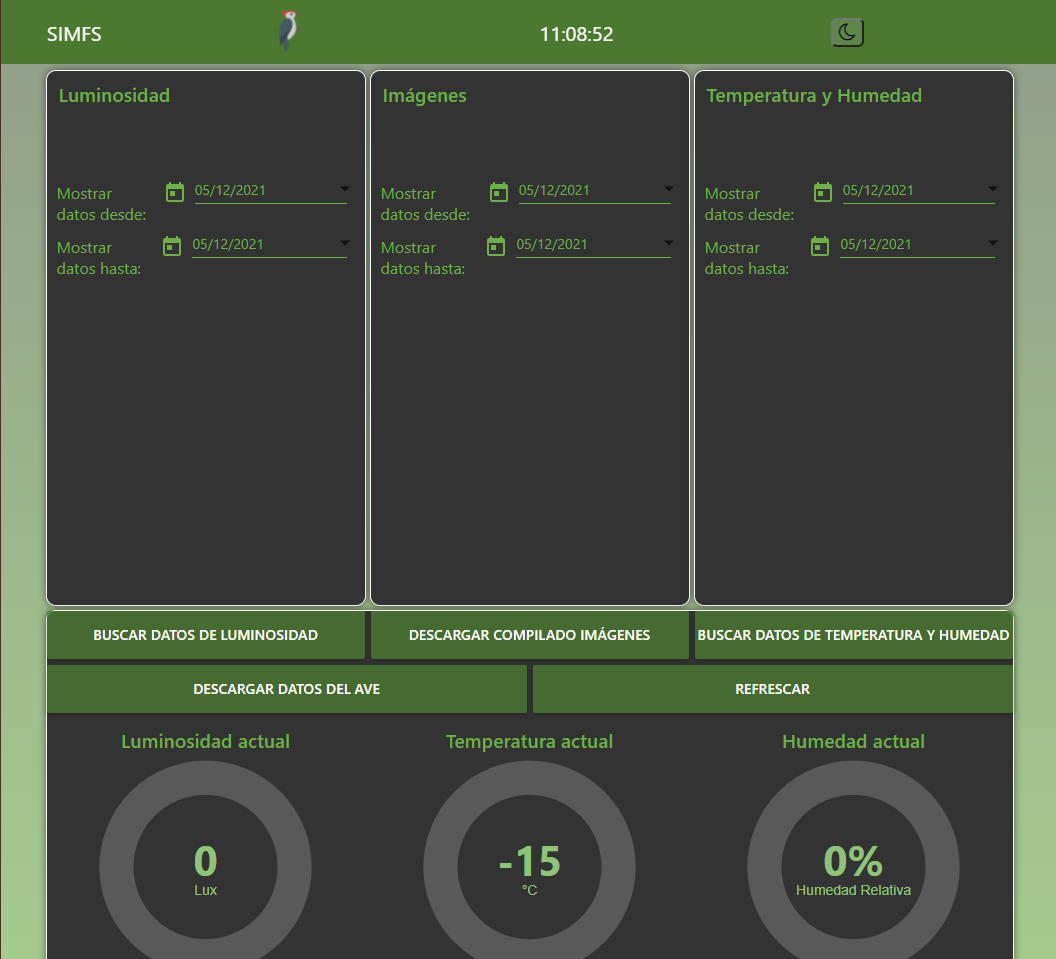
\includegraphics[width=0.7\linewidth]{ImagenesIngenieria de Detalle/Node-Red-Dark}
%	\label{fig:front_end}
%	\caption{Front end del servidor.}
%\end{figure}

\begin{figure}[H]
\centering
	\begin{subfigure}[b]{0.49\textwidth}
		\centering
		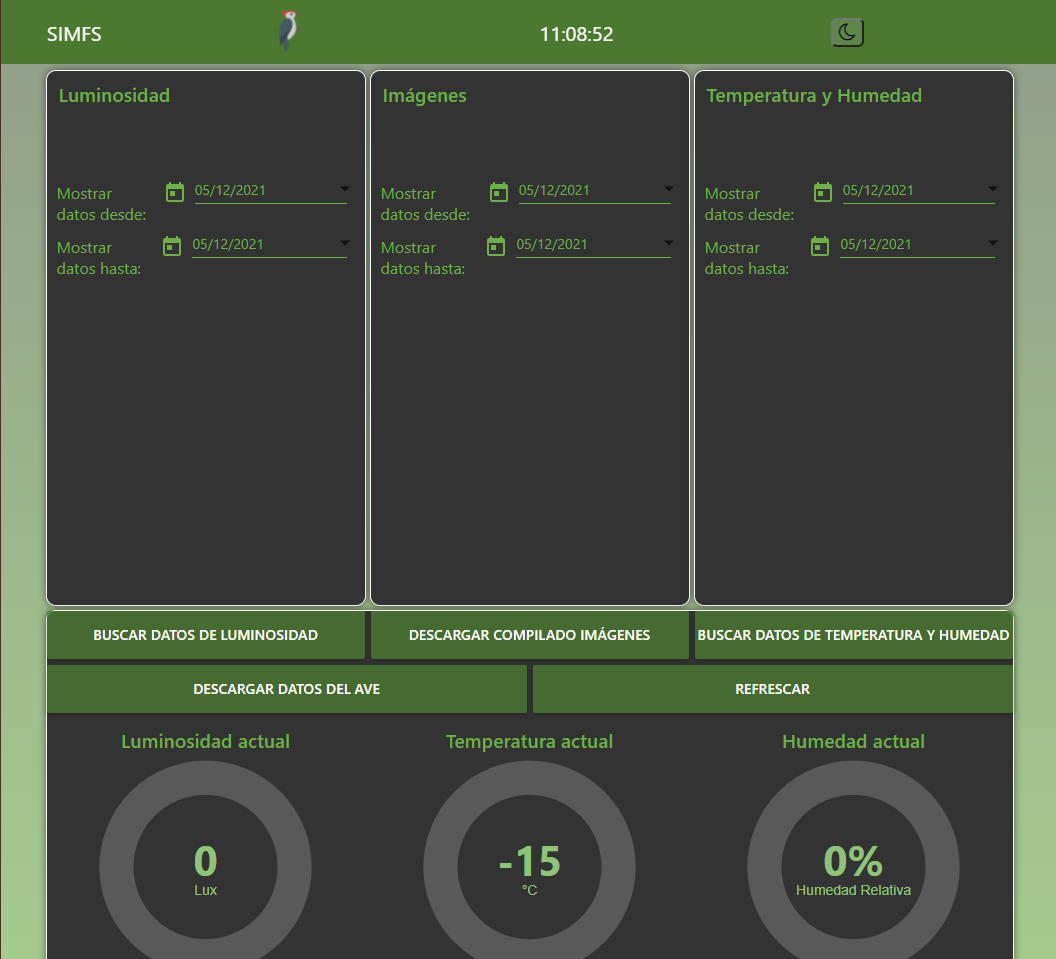
\includegraphics[width=\linewidth]{ImagenesIngenieria de Detalle/Node-Red-Dark}
	\label{fig:front_end_dark}
	\caption{Front end versión oscura.}
	\end{subfigure}
	%\hfill	
	\begin{subfigure}[b]{0.49\textwidth}
		\centering
		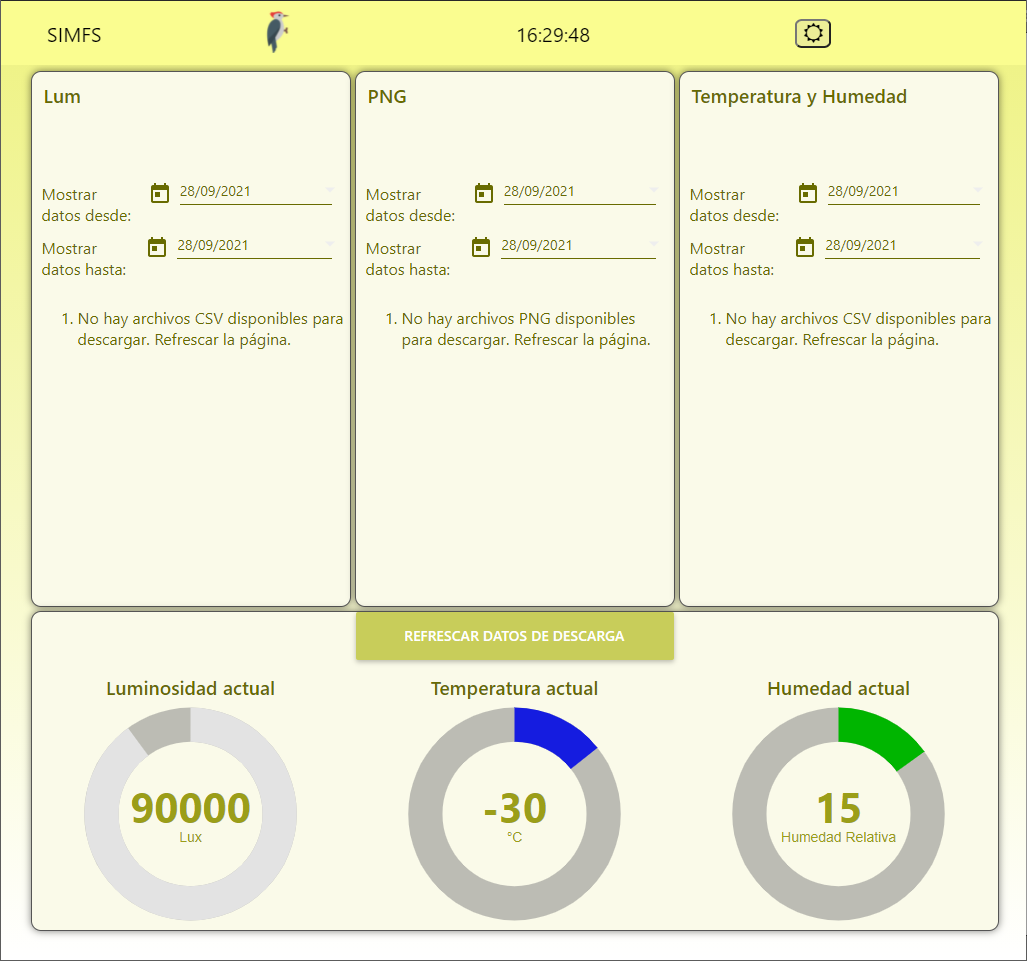
\includegraphics[width=\linewidth]{ImagenesIngenieria de Detalle/Node-Red-Light}
	\label{fig:front_end_light}
	\caption{Front end versión clara.}
	\end{subfigure}	
	\caption{Página del servidor a la cual accede el usuario.}
\end{figure}